\chapter*{Proposition 10}
\label{prop:10}

\begin{figure*}[ht]
    \begin{center}
    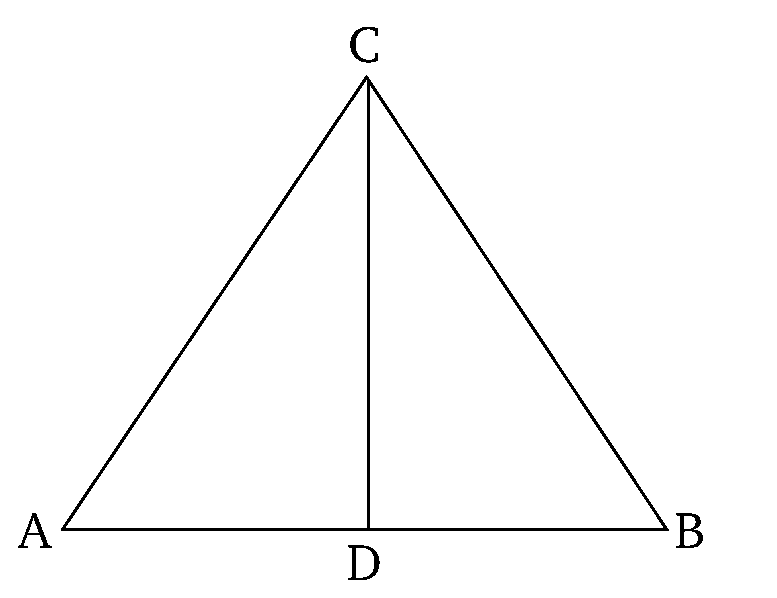
\includegraphics[width=0.5\linewidth]{figures/fig10e.eps}
    \label{fig:prop_10}
    \end{center}
\end{figure*}

To cut a given finite straight-line in half.

Let $AB$ be the given finite straight-line. So it is required to cut the
finite straight-line $AB$ in half.

Let the equilateral triangle $ABC$ have been constructed upon  ($AB$)
[Prop.~1.1], and let the angle $ACB$ have been cut in half by the
straight-line $CD$ [Prop.~1.9]. I say that the straight-line $AB$ has been
cut in half at  point $D$.

For since $AC$ is equal to $CB$, and $CD$ (is) common, the two (straight-lines) $AC$, $CD$
are equal to the two (straight-lines) $BC$, $CD$, respectively. And the angle $ACD$ is
equal to the angle $BCD$. Thus, the base $AD$ is equal to the base $BD$
[Prop.~1.4].

Thus, the given finite straight-line $AB$ has been cut in half at  (point) $D$. 
(Which is) the
very thing it was required to do.


\section*{Commentary}

\begin{proposition}\label{proposition_10}\lean{Elements.Book1.proposition_10}\leanok
    $A$ and $B$ are two distinct points on a line $AB$. There must exist a point $D$ between them, s.t., $|AD| = |DB|$.
\end{proposition}
\begin{proof}
    \uses{proposition_1,proposition_4,proposition_9'}\leanok
    See the original proof by Euclid.
\end{proof}
